\section{Flip Flop tipo T \label{sec:s2}}

\begin{center}
	\begin{minipage}{12cm}
		\begin{tcolorbox}[title=Actividad 2]
			El flip-flop tipo T es un circuito que se usa como base en la construcción de contadores. Se le llama tipo T por “\textit{Toggle}” es decir, cuando tiene aplicado un uno lógico a su entrada, el flip-flop invertirá el valor de su salida con el flanco de activación. Investigar su funcionamiento y describirlo. Simular el circuito.
		\end{tcolorbox}	
	\end{minipage}
\end{center}

El flip flop tipo T es un circuito lógico de entrada única que mantiene o alterna su salida según el estado de entrada. T es una abreviatura de \textit{Toggle} o conmutar, en español. La operación que realiza este tipo de flip flop es cambiar la salida del siguiente estado por el complemento del estado actual. A diferencia del flip flip tipo SR, el tipo T evita la aparición de un estado intermedio.\cite{oemsecrets_2021} Obviando el comportamiento del \textit{reset} que se implemente, el funcionamiento se da de la siguiente manera: si la entrada T presenta un nivel bajo ``0'', el dispositivo está en su modo de memoria (no presenta cambios), y si en la entrada T se encuentra un nivel alto ``1'', el dispositivo cambia de estado, es decir la salida adquiere el complemento del valor actual.\cite{Olmo} Es de utilidad en algunas aplicaciones como:

\begin{itemize}
	\item \textbf{División de frecuencia}: Se puede utilizar para dividir la frecuencia de una señal de reloj por dos, lo que lo hace útil en aplicaciones como relojes digitales y sintetizadores de frecuencia.
	\item \textbf{Multiplicación de frecuencia}: Se puede usar para multiplicar la frecuencia de una señal de reloj por dos, lo que lo hace útil en aplicaciones como sintetizadores de frecuencia y procesamiento de señales digitales.
	\item \textbf{Almacenamiento de datos}: Se puede emplear para almacenar un solo bit de datos, lo que lo hace útil en aplicaciones como registros de desplazamiento y dispositivos de memoria.
	\item \textbf{Contadores}: Se puede utilizar junto con otras puertas lógicas digitales para crear contadores binarios que pueden contar hacia arriba o hacia abajo según el diseño. Esto los hace útiles en aplicaciones en tiempo real como temporizadores y relojes. \cite{Anónimo_2023}
\end{itemize}

La visualización RTL del flip flop tipo T en Verilog se muestra en la \autoref{fig:ff_t_rtl}. Se observa que la implementación se hace instanciando un flip flop tipo D, pero colocando la señal T en la terminal ENA y usando un lazo de retroalimentación negativa entre la salida Q y la entrada D. Las simulaciones para el código en Verilog se visualizan en la \autoref{fig:ff_t_wave}, en donde se muestra que el dispositivo funciona de manera correcta, ya que en un inicio no se tiene un valor en la salida, hasta que se activa el \textit{reset}. Con el valor de la salida inicializado, se observa que al tener un valor alto en T, al siguiente flanco de subida del reloj se cambia el valor de la salida por su complemento.

En los Anexos se localiza la descripción del flip flop tipo T con \textit{reset} asíncrono. Se utilizó una lista sensible para el flanco de subida de la señal de reloj y el \textit{reset}. Dentro de esta estructura se empleó la sentencia \textit{if} para comparar el valor de RST:

\begin{itemize}
	\item Si es 1, se restablece el valor de la salida a 0. 
	\item Si es 0, continúa leyendo la sintaxis de código.
\end{itemize}

Y una sentencia \textit{else if} para comparar el valor de T:

\begin{itemize}
	\item Si es 1, se cambia el valor de la salida Q por el complemento del valor actual. 
	\item Si es 0, la salida no cambia y se mantiene su último valor.
\end{itemize}

\begin{figure}[ht]
	\centering
	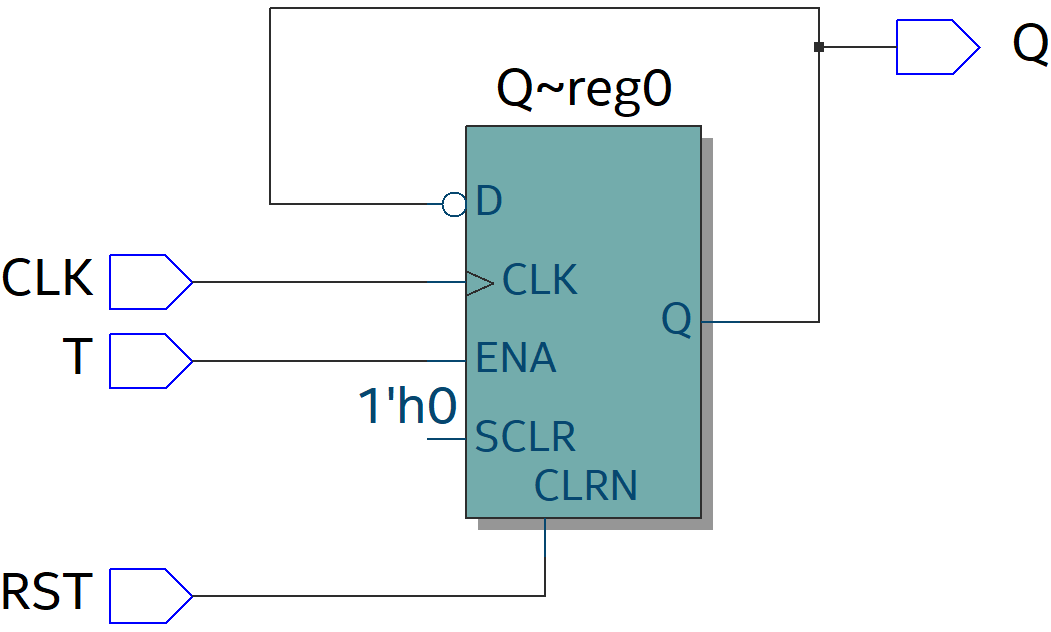
\includegraphics[scale=0.5]{FF_T_RTL.png}
	\caption{Diagrama RTL del flip flop tipo T con \textit{reset} asíncrono. \label{fig:ff_t_rtl}}
\end{figure}

\begin{figure}[ht]
	\centering
	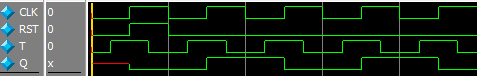
\includegraphics[scale=1.3]{FF_T_Wave.png}
	\caption{Simulación del flip flop tipo T con \textit{reset} asíncrono con el visor de formas de onda de ModelSim. \label{fig:ff_t_wave}}
\end{figure}